\section{Characterization}
\label{sec:motivation}
In this section, we explore the performance and utilization characteristics of LLM inference and draw key insights to guide the design of Splitwise. 

\myparagraph{Production traces}
%We use production traces taken from a large cloud provider, \cloudname.
We use production traces taken from two Azure LLM inference services on November 11$^{th}$ 2023. 
Our traces represent the most common scenarios in LLM inference today:
\emph{coding} and \emph{conversation}.
We have released a subset of our traces at \url{https://github.com/Azure/AzurePublicDataset}~\cite{azure_llm_trace}.
The traces we use for characterization are 20 minutes long and include the arrival time, input size (number of prompt tokens), and output size (number of output tokens).
%These traces contain a subset of the accesses from two of the most common scenarios in LLM inference today:
Due to customer privacy requirements (\eg, GDPR), we do not have visibility into the content of the prompts.
We instead use the production traces to guide the input and output sizes, where we send the input prompt with the required number of tokens, 
and force the model to generate the corresponding number of output tokens for each request.
Note that the text of the inputs prompts does not impact the performance metrics that we benchmark, since they depend only on the input and output sizes.
%Since this work does not care about LLM output quality, for each request in the trace, we use randomized text inputs that match the number of input tokens, and force the LLM to generate the right number of tokens as per the trace.
For this characterization, we do not reuse the KV-cache between requests to emulate a cloud service with security guarantees.


\myparagraph{Models}
\Cref{tab:models} shows the models that we evaluate.
Both BLOOM~\cite{scao2022bloom} and Llama2~\cite{hf_llama2} are state-of-the-art open source LLMs.
Both models are decoder-only, transformer-based models. 
We use the version of each model with the most parameters, since these versions are the most representative for production-class accuracy.
Unless stated otherwise, we run BLOOM-176B and Llama-70B on vLLM~\cite{vllm} on a machine with 8 H100~\cite{dgxh100} GPUs.

\begin{table}[t]
\centering
\footnotesize
\begin{tabular}{@{}cccc@{}}
\toprule
\textbf{Model}      & \textbf{\#Layers} & \textbf{Hidden size} & \textbf{\#Heads} \\ \midrule
% \textbf{OPT-30B}    & 48                & 7168                 & 56               \\
\textbf{Llama2-70B} & 80                &    8192              & 32                \\
%\textbf{ChatGPT-X*} &                   &                      &                  \\
\textbf{BLOOM-176B} & 70                & 14336                & 112              \\ \bottomrule
\end{tabular}
\caption{Models we evaluate and their parameters.}
\label{tab:models}
\end{table}


\subsection{Number of prompt and generated tokens}
To better understand our traces, we examine the distribution of the number of \emph{prompt input} and \emph{generated output} tokens.
\Cref{fig:prompt_sizes} shows the distribution of number of prompt tokens.
Since the coding LLM inference service is generally used to generate completions as the user is writing code, its input prompt can include large chunks of the code written so far.
%This shows in the distribution, as the median \emph{prompt} size is 1500 tokens.
Thus, it has a large median prompt size of 1500 tokens.
On the other hand, the conversation service has a wider range of input prompt tokens since it depends on the user.
The median number of prompt tokens for this trace is 1020 tokens.

\begin{figure}
    \centering
    \subfloat[Prompt input tokens.]{
        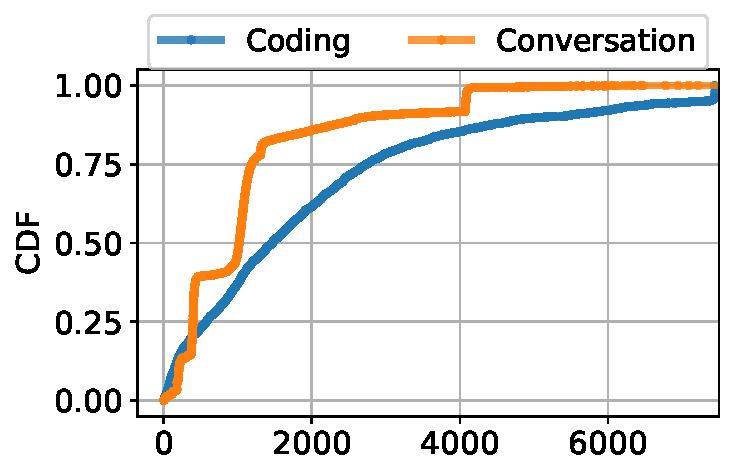
\includegraphics[width=0.48\columnwidth]{figures/characterization/trace/prompt_cdf.pdf}
        \label{fig:prompt_sizes}}
    \subfloat[Generated output tokens.]{
        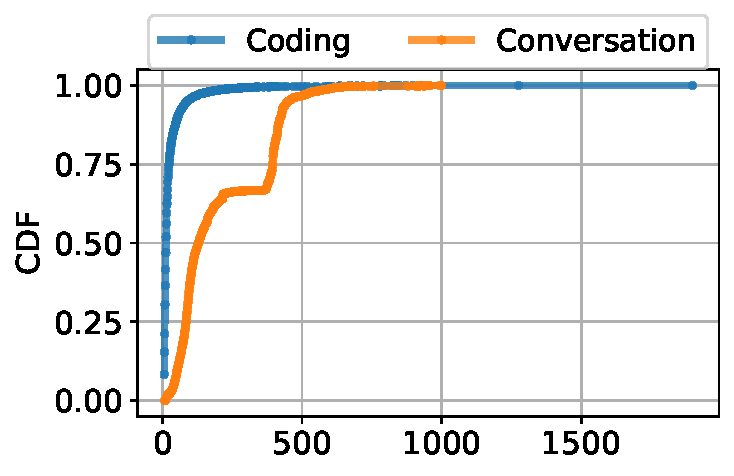
\includegraphics[width=0.48\columnwidth]{figures/characterization/trace/token_cdf.pdf}
        \label{fig:token_sizes}}
\caption{Distribution for prompt and generated tokens.}
    \label{fig:prompt_token_sizes} 
    %\vspace{-0.5cm}
\end{figure}

\Cref{fig:token_sizes} shows the distribution of the number of generated tokens.
Since the coding service typically only generates the next few words in the program as the user types, the median number of output token is 13 tokens.
On the other hand, the conversation service has an almost bimodal distribution, with a median of 129 tokens generated.

\insightparagraph{1}
Different inference services may have widely different prompt and token distributions.




\subsection{Batch utilization}

\begin{figure}
    \centering
    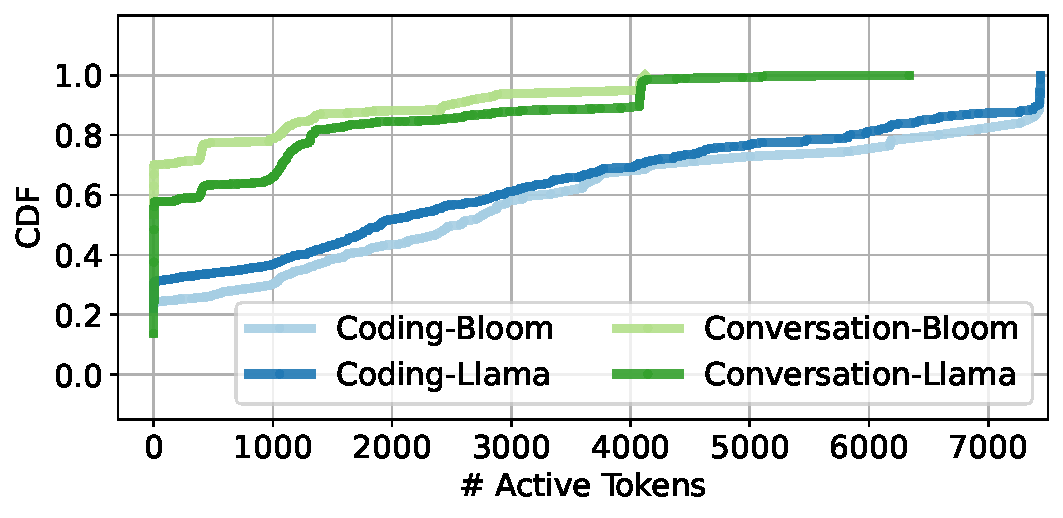
\includegraphics[width=0.7\columnwidth]{figures/characterization/vllm_pvt_distribution.pdf}
    \caption{Cumulative distribution of time spent with various active batched tokens.}
    \label{fig:pvt-distribution}
\end{figure}

To understand how much can these requests be batched, we measure how often machines run at a given batch size.
We use mixed continuous batching as shown in \Cref{fig:batching-gantt-chart}.
To fit into a single machine, we run a scaled-down version of the coding and conversation traces with 2 requests per second.

\Cref{fig:pvt-distribution} shows the distribution of the time spent by the machine running various number of active tokens in a batch.
Note that if a prompt of 100 tokens is running in its prompt phase, we count the active tokens as 100.
However, once the request is in the token phase, we count it as one active token, since the tokens are generated one at a time (assuming a beam search size of one~\cite{vllm}).
We find that most of the time (60--70\%) for conversation is spent running only 20 tokens or fewer. 
Since the coding service has very few output tokens, it experiences even worse batching in the token phase and runs with a single token for more than 20\% of the time.
Both the LLMs show very similar trends.

\insightparagraph{2}
Mixed continuous batching spends most of the time with very few active tokens batched.

\begin{figure}
    \centering
    \subfloat[TTFT by prompt size.]{
        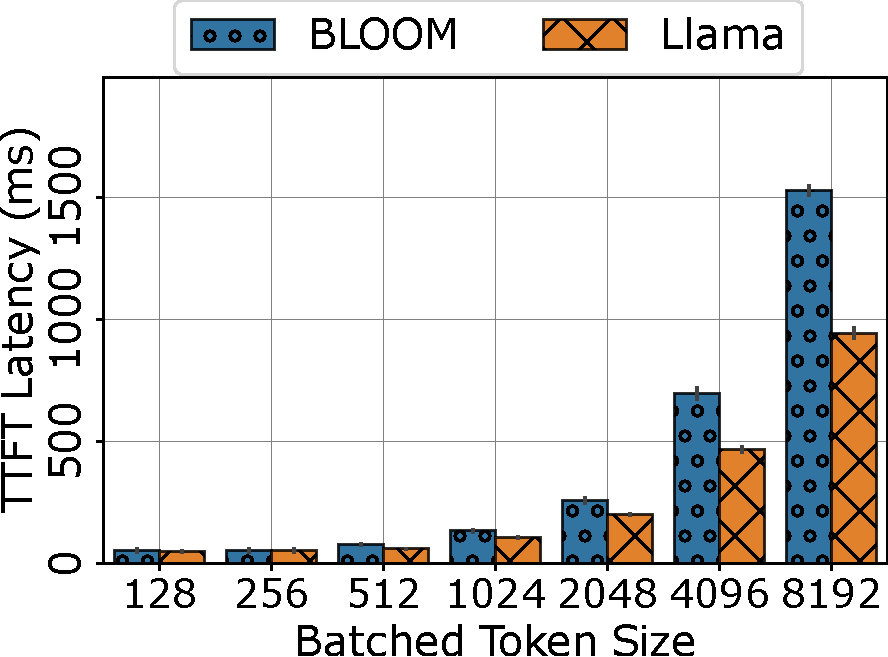
\includegraphics[width=0.32\columnwidth]{figures/characterization/prompt/h100-input_size-latency}
        \label{fig:characterization_TTFT}}
    \subfloat[TBT by batch size.]{
        
\includegraphics[width=0.32\columnwidth]{figures/characterization/token/h100-batch_size-latency}
        \label{fig:characterization_TBT}}
    \subfloat[Latencies on prod traces (no batching).]{
        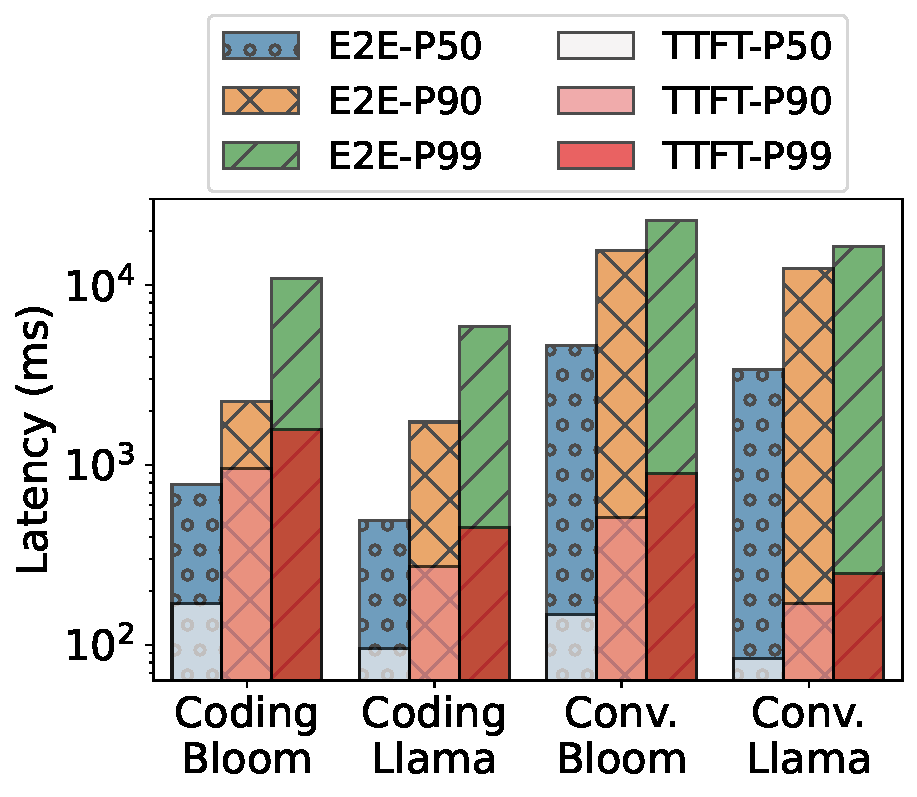
\includegraphics[width=0.32\columnwidth]{figures/characterization/vllm_pvt_perf}
        \label{fig:characterization_E2E}}            
\caption{TTFT, TBT, and E2E for BLOOM-176B and Llama-70B on DGX-H100.}
    \label{fig:char_TTFT_TBT_E2E} 
    %\vspace*{-0.5cm}
\end{figure}

\subsection{Latency}


\myparagraph{TTFT}
\Cref{fig:characterization_TTFT} shows the impact of the number of prompt tokens on TTFT.
The range of sizes was chosen based on the coding and conversation traces.
We find that TTFT for both models grows almost linearly as the prompt size increases.
This behavior is due to the prompt phase having high GPU utilization and being computationally bound.

\myparagraph{TBT}
\Cref{fig:characterization_TBT} shows the impact of forcefully batching the output tokens of different requests together on the TBT.
We observe very little impact on TBT as the batch size grows.
With a batch size of 64, there is only $2\times$ impact on TBT.
%Since the token phase is memory-bound, we see this pattern.

\myparagraph{E2E}
\Cref{fig:characterization_E2E} shows various percentiles of E2E latency for both models, with no batching.
The variability between the request input and output sizes is apparent.
Furthermore, we see that most of the E2E time is spent running the token phase.
This holds true even for the coding trace, where prompt sizes are large and generated tokens few. 
%This further explains the findings in \Cref{fig:pvt-distribution}.
In fact, we find that for BLOOM-176B, a prompt phase with 1500 input tokens takes the same time as token phase with only 6 output tokens.

\insightparagraph{3}
For most requests, the majority of the E2E time is spent in the token generation phase.

\begin{figure}
    \centering
    \subfloat[Prompt phase.]{
        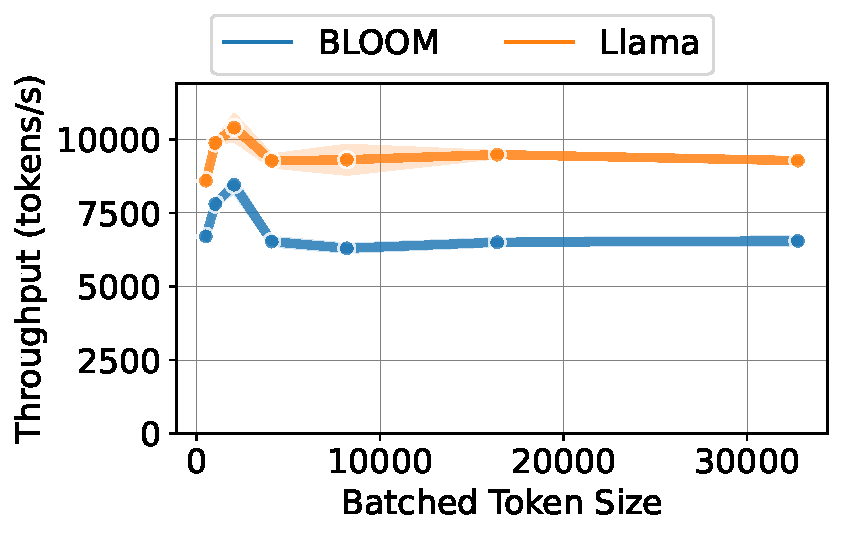
\includegraphics[width=0.48\columnwidth]{figures/characterization/prompt/h100-batch_size-throughput.pdf}
        \label{fig:char_tput_prompt}}
    \subfloat[Token generation phase.]{
        
\includegraphics[width=0.48\columnwidth]{figures/characterization/token/h100-batch_size-throughput.pdf}
        \label{fig:char_tput_token}}
    \caption{Impact of batching on the throughput for the 2 LLMs.}
    \label{fig:char_tput} 
\end{figure}



\subsection{Throughput}
\Cref{fig:char_tput} shows the impact of batching on the throughput (measured as tokens per second).
For the prompt phase, we define the throughput as the number of prompt input tokens that are processed per second.
We see that the throughput decreases after 2048 prompt tokens, which corresponds to a batch size of less than 2 for the median prompt sizes from the traces.
On the other hand, \Cref{fig:char_tput_token} shows that the throughput in the token phase keeps increasing with batching until 64 batch-size, at which point, the machine runs out of memory.


\insightparagraph{4}
The prompt phase batch size should be limited to ensure good performance.
In contrast, batching the token generation phase yields high throughput without any downside.

\begin{figure}
    \centering
     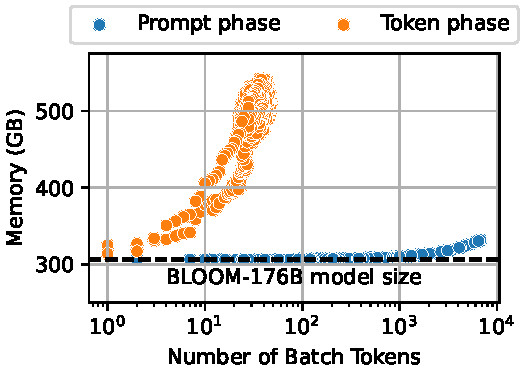
\includegraphics[width=0.60\columnwidth]{figures/characterization/memory_vs_batch_tokens_bloom-176b_conv70.pdf}
    \caption{Required memory with batching in prompt/token phases.}
    \label{fig:char_memory}
    %\vspace*{-0.5cm}
\end{figure}

\subsection{Memory utilization}
During an LLM inference, the GPU memory is used to host the model weights and activations, as well as the KV caches (\Cref{sec:kvcachebg}).
As the number of tokens in a batch increase, the memory capacity required for the KV cache also increases.
\Cref{fig:char_memory} shows the memory capacity utilization during each phase as the number of tokens in the batch increases.
During the prompt phase, the input prompt tokens generate the KV cache.
During the output token phase, \emph{each} active generated token that is being processed accesses the KV cache of its \emph{entire context} so far.

\insightparagraph{5}
Batching during the prompt phase is compute-bound, whereas the token phase is limited by memory capacity.

\begin{figure}
    \centering
    \subfloat[Prompt phase.]{
        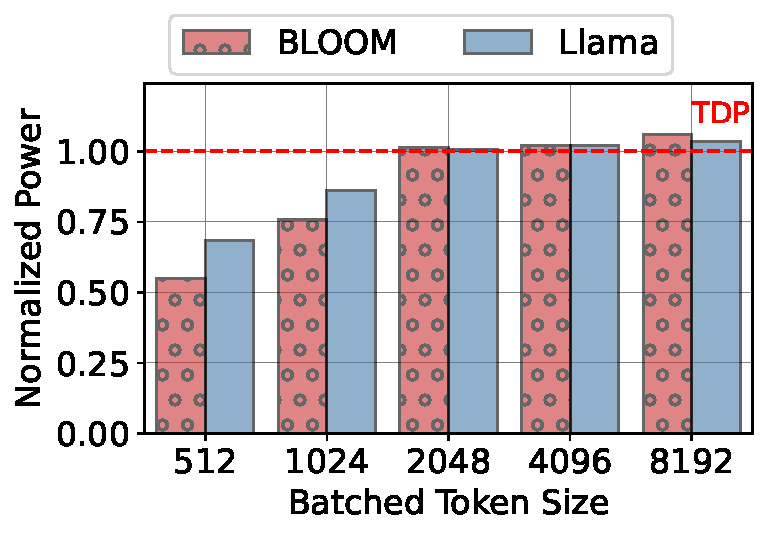
\includegraphics[width=0.48\columnwidth]{figures/characterization/prompt/h100-batch_size-power.pdf}
        \label{fig:char_power_prompt}}
    \subfloat[Token generation phase.]{
        
\includegraphics[width=0.48\columnwidth]{figures/characterization/token/h100-batch_size-power.pdf}
        \label{fig:char_power_token}}
    \caption{Maximum and mean power utilization varying the batching size.
    }
    \label{fig:char_power}
    %\vspace{-0.5cm}
\end{figure}

\begin{figure}[t]
    \centering
    \subfloat[Prompt phase.]{
        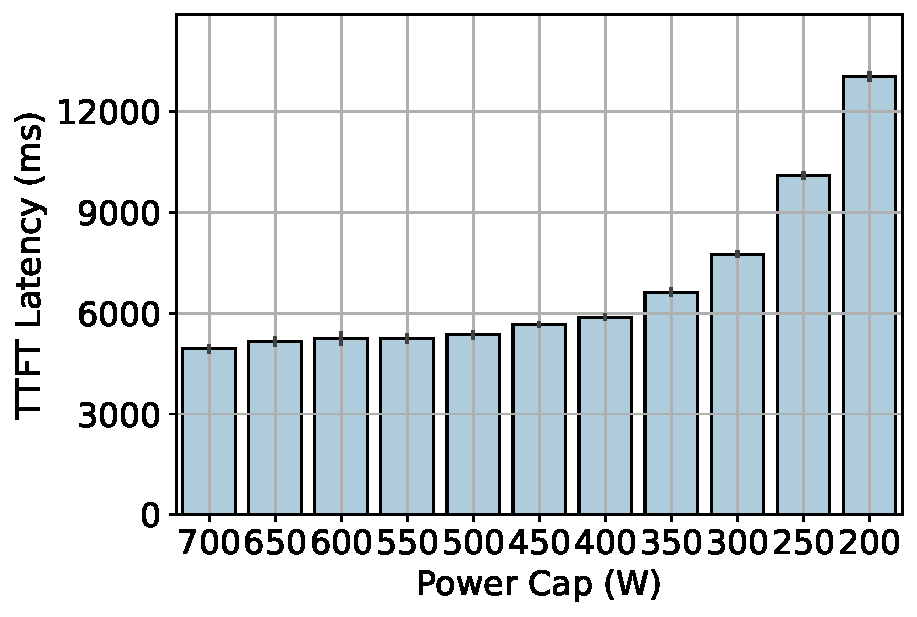
\includegraphics[width=0.48\columnwidth]{figures/characterization/prompt/power_capping.pdf}
        \label{fig:char_power_cap_prompt}}
    \subfloat[Token generation phase.]{
        
\includegraphics[width=0.48\columnwidth]{figures/characterization/token/power_capping.pdf}
        \label{fig:char_power_cap_token}}
    \caption{Impact of power cap on the prompt and token generation latency with the maximum batch size possible.
    }
    \label{fig:char_powercap}
\end{figure}



\subsection{Power utilization}
When hosting machines, cloud providers need to consider the peak power draw, which has direct impact in the datacenter cost~\cite{barroso2018_Datacenter}.
This is especially important when building GPU clusters, since GPUs consume much higher power than regular compute machines~\cite{patel2024llmpower,patel2023towards}.
\Cref{fig:char_power} shows the GPU power draw normalized to the thermal design power (TDP) when running prompt and token generation phases.
Since the the prompt phase is compute intensive, its power draw increases with batch size.
On the other hand, the token phase is memory bound and its power draw does not vary when increasing the number of tokens to process.

Providers can cap the power usage of the machines to reduce the peak power.
\Cref{fig:char_powercap} shows the impact to latency when increasing the power caps for both prompt and token phases.
The prompt phase is highly sensitive to the power cap and the latency increases substantially.
On the other hand, the token generation phase incurs almost no latency impact when power capping by over 50\% (\ie, 700 to 350W).

\insightparagraph{6}
While the prompt phase utilizes the power budget of the GPU efficiently, the token phase does not.


\begin{table}[t]
\centering
\footnotesize
\begin{tabular}{@{}ccccccc@{}}
\toprule
                      &\multicolumn{3}{c}{\textbf{Coding}} & \multicolumn{3}{c}{\textbf{Conversation}}\\
                      & \textbf{A100}   &\textbf{H100}  &\textbf{Ratio}      &\textbf{A100}      &\textbf{H100} &\textbf{Ratio}\\\midrule                      
\textbf{TTFT}         & 185 ms   & 95 ms  & 0.51$\times$ & 155 ms  & 84 ms   & 0.54$\times$ \\
\textbf{TBT}          & 52 ms    & 31 ms  & 0.70$\times$ & 40 ms   & 28 ms   & 0.70$\times$ \\
\textbf{E2E}          & 856 ms   & 493 ms & 0.58$\times$ & 4957 ms & 3387 ms & 0.68$\times$ \\
\textbf{Cost~\cite{coreweave}} & \$0.42 & \$0.52 & 1.24$\times$ & \$2.4  & \$3.6 & 1.5$\times$ \\
\textbf{Energy}       & 1.37 Whr & 1.37 Whr & 1$\times$  & 7.9 Whr   & 9.4 Whr    & 1.2$\times$ \\
\bottomrule
\end{tabular}
\caption{P50 request metrics on A100 vs. H100 without batching on Llama-70B.}
\label{tab:a100h100results}
%\vspace{-0.5cm}
\end{table}


\subsection{GPU hardware variations}
Given the different characteristics of prompt and token generation phases, we measure the performance impact on the two from running on different hardware.
\Cref{tab:a100_vs_h100_specs} shows the specifications for DGX-A100~\cite{nvidia_dgx_a100} and DGX-H100~\cite{dgxh100}. The memory-to-compute ratio favors A100 over H100.
Table~\ref{tab:a100h100results} shows our findings. 
We see a lower performance impact on the token generation phase (TBT) as compared to the Prompt phase (TTFT).
Since coding requests are dominated by prompt phase, by having very few generated tokens, the E2E latency impact from A100 is worse on coding than conversation.
Furthermore, we see that A100 has better or equal inference cost and energy overall compared to H100.

\insightparagraph{7}
Token generation can be run on less compute-capable hardware for better Perf/W and Perf/\$ efficiencies.



